\documentclass[11pt,oneside]{article}	%use"amsart"insteadof"article"forAMSLaTeXformat
\usepackage{geometry}		%Seegeometry.pdftolearnthelayoutoptions.Therearelots.
\geometry{letterpaper}		%...ora4paperora5paperor...
%\geometry{landscape}		%Activateforforrotatedpagegeometry
%\usepackage[parfill]{parskip}		%Activatetobeginparagraphswithanemptylineratherthananindent
\usepackage{graphicx}				%Usepdf,png,jpg,orepsßwithpdflatex;useepsinDVImode
								%TeXwillautomaticallyconverteps-->pdfinpdflatex		
\usepackage{amssymb}
\usepackage{hyperref}

%----macros begin---------------------------------------------------------------
\usepackage{color}
\usepackage{amsthm}

\def\conv{\mbox{\textrm{conv}\,}}
\def\aff{\mbox{\textrm{aff}\,}}
\def\E{\mathbb{E}}
\def\R{\mathbb{R}}
\def\Z{\mathbb{Z}}
\def\tex{\TeX}
\def\latex{\LaTeX}
\def\v#1{{\bf #1}}
\def\p#1{{\bf #1}}
\def\T#1{{\bf #1}}

\def\vet#1{{\left(\begin{array}{cccccccccccccccccccc}#1\end{array}\right)}}
\def\mat#1{{\left(\begin{array}{cccccccccccccccccccc}#1\end{array}\right)}}

\def\lin{\mbox{\rm lin}\,}
\def\aff{\mbox{\rm aff}\,}
\def\pos{\mbox{\rm pos}\,}
\def\cone{\mbox{\rm cone}\,}
\def\conv{\mbox{\rm conv}\,}
\newcommand{\homog}[0]{\mbox{\rm homog}\,}
\newcommand{\relint}[0]{\mbox{\rm relint}\,}

%----macros end-----------------------------------------------------------------

\title{LAR-ABC, a representation of architectural geometry \\
{\Large From concept of spaces, to design of building fabric, to construction simulation}
\footnote{This document is part of the \emph{Linear Algebraic Representation with CoChains} (LAR-CC) framework~\cite{cclar-proj:2013:00}. \today}
}
\author{Alberto Paoluzzi \and Enrico Marino \and Federico Spini}
%\date{}							%Activatetodisplayagivendateornodate

\begin{document}
\maketitle
%\nonstopmode

\begin{abstract}
This paper discusses the application of LAR (Linear Algebraic Representation) scheme~\cite{Dicarlo:2014:TNL:2543138.2543294} to the whole architectural design process, from initial concept of spaces, to the additive manufacturing of design models, to the meshing for CAE analysis, to the detailed design of components of building fabric, to the BIM processing of quantities and costs. LAR (see, e.g. [1]) is a novel general and simple representation scheme for geometric design of curves, surfaces and solids, using simple, general and well founded concepts from algebraic topology. 
LAR supports all topological incidence structures, including enumerative (images), decompositive (meshes) and boundary (CAD) representations. It is dimension-independent, and not restricted to regular complexes. Furthermore, LAR enjoys a neat mathematical format, ��being based on chains, the domains of discrete integration, and cochains, the discrete prototype of differential forms, so naturally integrating the geometric shape with the supported physical properties. 
The LAR representation find his roots in the design language Plasm~\cite{Paoluzzi2003a}, and is currently embedded in python and javascript, providing the designer with powerful and simple tools for a geometric calculus of shapes. In this paper we introduce the motivation of this approach, discussing how it compares to other mixed-dimensionality representations of geometry and is supported by open-source software projects. We also discuss simple examples of use, with reference to various stages of the design process.
\end{abstract}

\newpage
\tableofcontents
\newpage

%-------------------------------------------------------------------------------
%===============================================================================
\section{Introduction}\label{sec:intro}
%===============================================================================
%-------------------------------------------------------------------------------
% 2 column
Looking for simplicity. 
Form and function. Who comes first?
CAD is evolving with the net.
Algebraic geometry on graphics processors.

%-------------------------------------------------------------------------------
%===============================================================================
\section{Linear Algebraic Representation}\label{sec:lar}
%===============================================================================
%-------------------------------------------------------------------------------
\subsection{Representation scheme}
%-------------------------------------------------------------------------------
% 1 column
A foundational concept. Mapping from mathematical models to computer representations. 
Taxonomy: decompositive, enumerative, boundary, procedural representations.
The de-facto standard of PLM systems: non-manifold data structures + NURBS. 
Old, expensive, and inflexible.
Towards big geometric data. The need for rethinking the foundations. 
Algebraic geometry is here to stay. Sparse matrices and GPGPU.

%-------------------------------------------------------------------------------
\subsection{Topological operations}
%-------------------------------------------------------------------------------
% 1 column
Space decompositions. Chains as subsets of spaces. Cochains as fields over chains. Geometric integration: pairing of chains and cochains. Homology and cohomology. Boundary and coboundary operators. A single SpMV multiplication to compute the boundary of any chain of spaces.
Transposition and coboundary. Coboundary and operators of vector analysis: gradient, curl, divergenze, and Laplacian. Integration of geometry and physics through topological structures. Topological queries. The $d$-star of every cell. Decomposition of big structures and distributed computing.

%-------------------------------------------------------------------------------
\subsection{Models and structures}
%-------------------------------------------------------------------------------
% 2 columns
Model = Topology + Geometry. Model as embedded topology. Topology as the list of higher-dimensional cells of a space decomposition. The classical representation of cells via the list of their vertices. Composition of linear operators as the product of their matrices.
Fast transposition and product operations via GPGPU and OpenCL. Structures as hierarchical aggregation of space-instanced models and/or other structures. The representation of structures as ordered sequences of strictres, models and operators. Data Base of structures. The traversal of structures at run-time.

%===============================================================================
\section{LAR for Architecture, Building and Construction}\label{sec:abc}
%===============================================================================
%-------------------------------------------------------------------------------
\subsection{Architectural structures: the organisation of spaces}
%-------------------------------------------------------------------------------
% 1 column
Organic or rational architecture? Form from function or vice-versa? In either case, space units produce organised assemblies of spaces with more or less specialised functions. In set-theoretical terms, they provide either a partitioning or a covering of the building space. At the very end, an architectural design defines a topology of the space, as a collection of subsets (of space), closed with respect to finite intersection and union. 

In practical terms, the design concept will result in a cellular decomposition of the space, where elementary space units, either open or closed or partially open, establish pairwise adjacency relations; even before of any concrete embedding, i.e. even before that a global shape is envisioned by the architect. 

In the majority of cases, the geometric embedding of the design topology will produce a partitioning of space with plane or curved surfaces, and some horizontal or vertical composition of use patterns. In common building and construction, most of the separating surfaces will be either horizontal or vertical, but different arrangements of space cells are possible.

LAR-ABC requires that the topology is first defined hierarchically, producing finally a space plan subdivided by layers, where the junctions of at least three separating surfaces are identified and numbered. The simplest data definition is, of course, via the production of planar architectural drawings embedded in a common reference system.

%-------------------------------------------------------------------------------
\subsection{Models, structures, assemblies}
%-------------------------------------------------------------------------------

In LAR-ABC we make a distinction between geometric \emph{models}, \emph{structures}, and \emph{assemblies}. Some terminology and definitions are given below.

\paragraph{Geometric model}
A geometric \emph{model} is a pair (\emph{geometry},\emph{topology}) in a given coordinate system, where  \emph{topology} is the LAR specification of highest dimensional cells of a cellular decomposition of the model space, and \emph{geometry} is specified by the coordinates of \emph{vertices}, the spatial embedding of 0-cells of the cellular decomposition of space. From a coding viewpoint, a model is either an instance of the \texttt{Model} class, or simply a pair (\texttt{vertices}, \texttt{cells}), where \texttt{vertices} is a two-dimensional array of floats arranged by rows, and where the number of columns (i.e.~of \emph{coordinates}) equals the dimension $n$ of the embedding Euclidean space $\E^n$. Similarly, \texttt{cells} is a list of lists of vertex indices, where every list of indices corresponds to one of $d$-dimensional \emph{cells} of the space partition, with $d\leq n$.

\paragraph{Structure}
A \emph{structure} is the LAR representation of a hierarchical organisation of spaces into substructures, that may be organised into lower-level substructures, and so on, where each part \emph{may} be  specified in a \emph{local coordinate system}. Therefore, a structure is given as an \emph{(ordered) list of substructures and transformations} of coordinates, that apply to all the substructures following in the same list. A structure actually represents a \emph{graph of the scene}, since a substructure may be given a name, and referenced more than one time within one or more other structures.  The \emph{structure network}, including references, can be seen as an acyclic directed multigraph. In coding term, a structure is an instance of the \emph{Struct} class, whose parameter is a list of either other structures, or models, or transformations of coordinates, or references to structures or models.

\paragraph{Assembly}
An assembly is an \emph{(unordered) list of models} all \emph{embedded in the same coordinate space}, i.e.~all using the same coordinate system (the \emph{world coordinate system}). A assembly may be either defined by the user as a list of models, or automatically generated by the \emph{traversal} of a structure network. At traversal time, all the traversed structures and models are transformed from their local coordinate system to the world coordinates, that correspond to the coordinate frame of the root of the traversed network, i.e.~to the first model of the structure passed as argument to the \texttt{evalStruct} function, that implements the traversal algorithm. In few words, we can say that an assembly is the linearised version of the traversed structure network, where all the models are using the world coordinate system.


%-------------------------------------------------------------------------------
\subsection{Building objects: components and assemblies}
%-------------------------------------------------------------------------------
When the project plan is accepted by the client, giving a definite shape to the first architectural concept, it is usually a 2.5D model, made by opaque or transparent 2D surfaces embedded in 3D space. 

In this stage, LAR-ABC allows for the computation of every topological or geometrical property of interest, including the evaluation of the surface of the building envelope and its partitioning into subsets with different thermal requirements, as well as the computation of the internal volume, and its partitioning into any classes of internal space, and will grant any other geometric computation or simulation (for example of the thermal behaviour) of possible interest for the architect or the client.

The LAR description of the topology and its geometric embedding, defined by the position vectors of vertices or control points of the surfaces, makes possible to (mostly) automatically generate a first 3D model of the physical construction, i.e.~of the concrete instances of building components.

This (semi-)automatic transformation from a 2.5D model formed by surfaces to a 3D model formed by assemblies of solid objects, is obtained using the boundary operator, that allow to discriminate between the various subsystems of the building fabric, i.e.~between the horizontal and vertical enclosures, the horizontal and vertical partitions of the interior, the elements of horizontal and vertical communications, and so on, as we show in Section~\ref{sec:examples}. 

%-------------------------------------------------------------------------------
\subsection{Construction process: computer simulation}
%-------------------------------------------------------------------------------
% 1 column
Some general information about the technologies to be used in the construction  allows to visualise as a computer animation the construction process embedded in time.
Starting to the specification of the hierarchical assemblies and from some additional information about the precedence relation between the construction activities, a construction PERT, giving the time schedule of the building erection. In the final subsection of Section~\ref{sec:examples} we discuss a simplified example.
Of course, a preliminary but informed guess of quantities and costs ban be also produced from the 3D solid model. 


%-------------------------------------------------------------------------------
%===============================================================================
\section{Examples}\label{sec:examples}
%===============================================================================
%-------------------------------------------------------------------------------
\subsection{Housing design}
%-------------------------------------------------------------------------------

A simple example of housing design is discussed in this section.
The concept of the dwelling produced by using a vectorial drawing program, is shown in Figure~\ref{fig:concept}. The input file is parsed, producing the LAR \texttt{model} given in the script below, as a pair \texttt{V,FV} of vertices \texttt{V} and 2-cells \texttt{FV}.


\begin{figure}[htbp] %  figure placement: here, top, bottom, or page
   \centering
   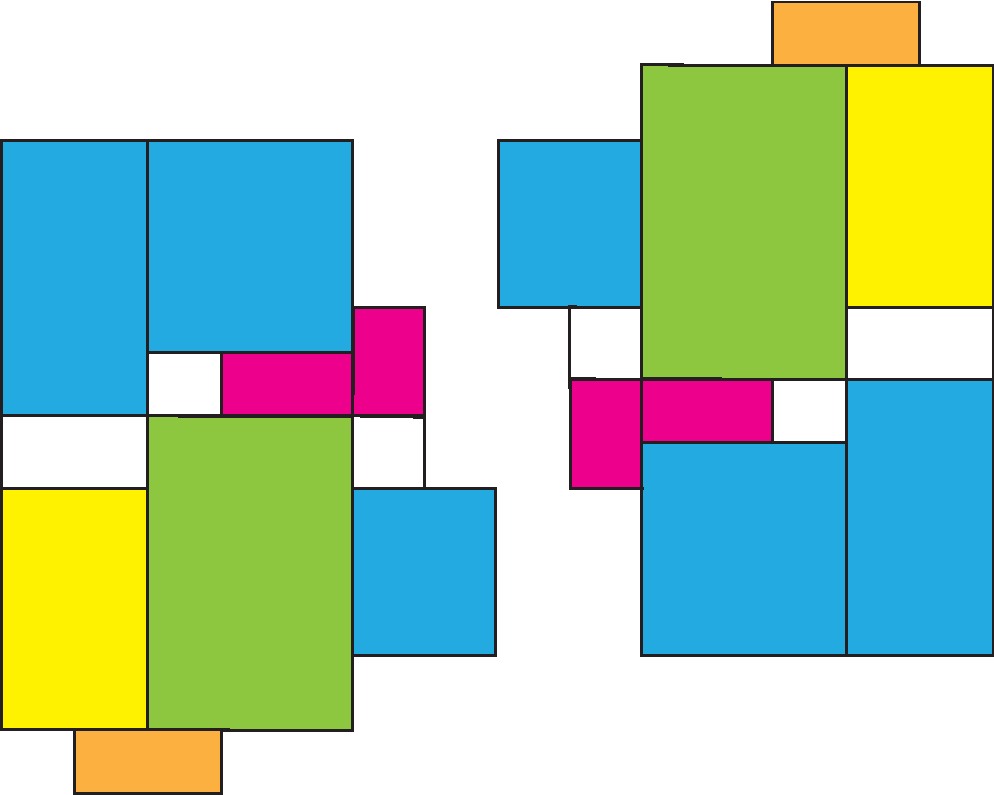
\includegraphics[width=0.37\linewidth]{images/concept2} \hfill
   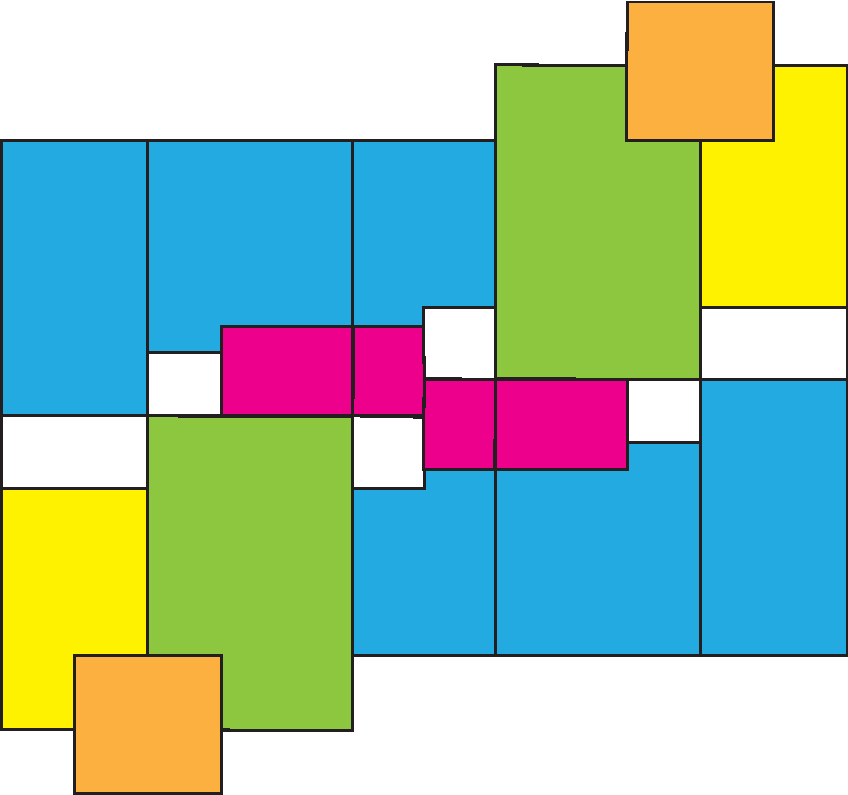
\includegraphics[width=0.32\linewidth]{images/concept3} \hfill
   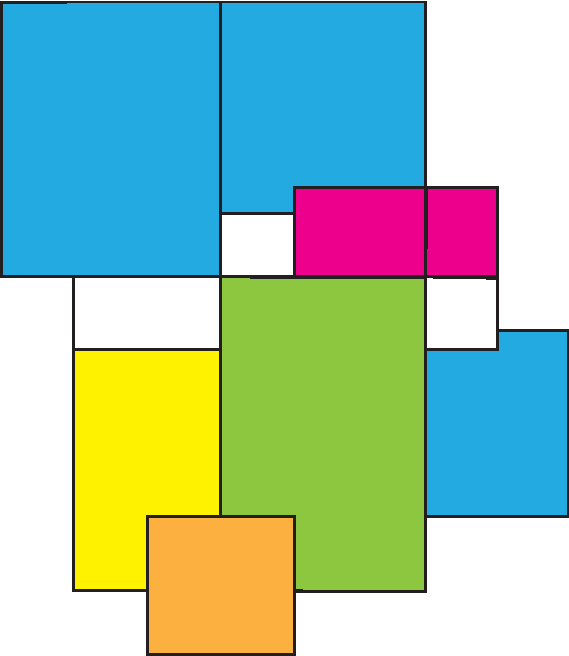
\includegraphics[width=0.215\linewidth]{images/concept0} 
   
   \caption{Concept design. living/eating area (green/yellow); bedrooms (cyan), lavatories (magenta); entrance (white).}
   \label{fig:concept}
\end{figure}

\subsubsection{LAR model input}


\paragraph{Input of the dwelling concept}
The vertices list \texttt{V} contains pairs of coordinates within a local reference frame. The 2-cell list \texttt{FV}  of references to vertices is given counterclockwise, in order to automatically get a complete LAR representation of topology, i.e.~the pair \texttt{FV, EV} of 2-cells and 1-cells.

%-------------------------------------------------------------------------------
@D Input of LAR architectural plan
@{
V = [[3,-3],
[9,-3],[0,0],[3,0],[9,0],[15,0],
[3,3],[6,3],[9,3],[15,3],[21,3], 
[0,9],[6,9],[15,9],[18,9],[0,13],
[6,13],[9,13],[15,13],[18,10],[21,10], 
[18,13],[6,16],[9,16],[9,17],[15,17],
[18,17],[-3,24],[6,24],[15,24],[-3,13]]
FV = [
[22,23,24,25,29,28], [15,16,22,28,27,30], [18,21,26,25], 
[13,14,19,21,18], [16,17,23,22], [11,12,16,15],
[9,10,20,19,14,13], [2,3,6,7,12,11], [0,1,4,8,7,6,3],
[4,5,9,13,18,17,16,12,7,8],[17,18,25,24,23]]
dwelling = [V,FV]
@}
%-------------------------------------------------------------------------------

\subsubsection{From faces to list of edges}

Some transformations of 2D data are given In this section. 

\paragraph{From faces FV to list of edges EV}
The \texttt{face2edge} operator takes every consecutive pair of vertex indices from each face and return such list of pairs (i.e.~the \texttt{EV} relation), filtered from double instances.
%-------------------------------------------------------------------------------
@D From faces FV to list of edges EV
@{def face2edge(FV):
	""" From faces to list of edges """
	edges = AA(sorted)(CAT([TRANS([face, face[1:]+[face[0]]]) for face in FV]))
	return AA(eval)(set(AA(str)(edges)))
@}
%-------------------------------------------------------------------------------

\paragraph{From LAR model to list of polylines}
The function \texttt{lar2polylines}
transform a LAR model into a list of polylines, i.e.~of (closed) lists of 2D points, where the last point coincides with the first one.
%-------------------------------------------------------------------------------
@D From faces FV to list of edges EV
@{def lar2polylines (model):
	""" From LAR model to list of polylines """
	V,FV = model
	return [[V[v] for v in cell]+[V[cell[0]]] for cell in FV]
@}
%-------------------------------------------------------------------------------

\subsubsection{Partitioning the 1-cells}

The subdivision of 1-cells of the complex between boundary cells and interior cells is executed by computing the boundary operator $\partial_2$, and multiplying it by the coordinate representation $\mathbf{1}$ of the 2D basis of cells. 


\begin{figure}[htbp] %  figure placement: here, top, bottom, or page
   \centering
   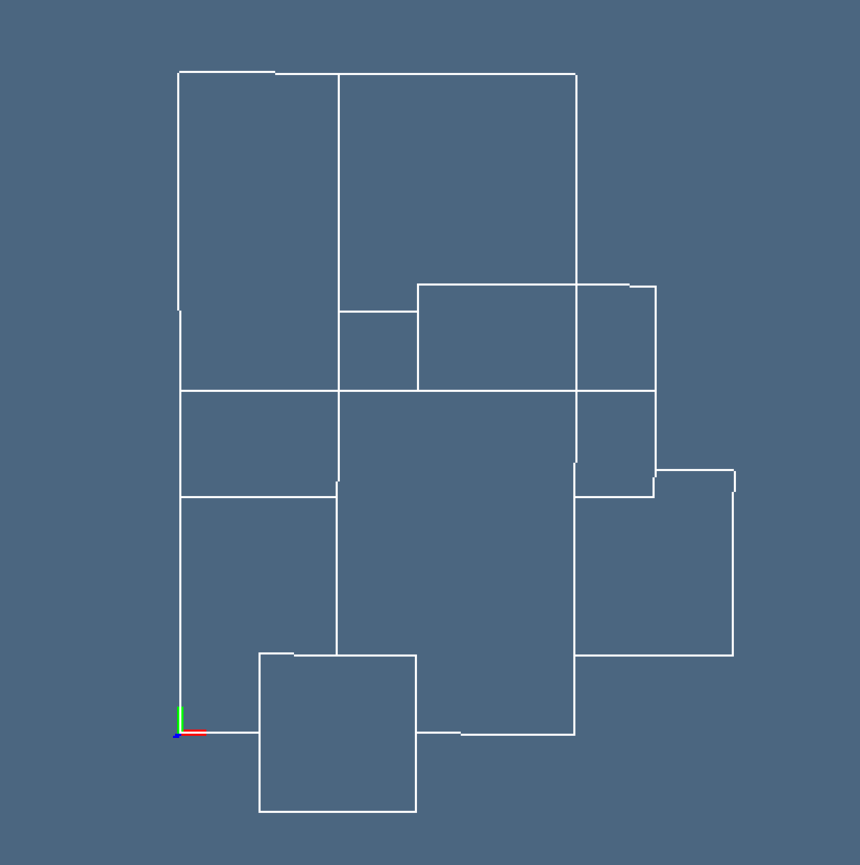
\includegraphics[height=0.243\linewidth,width=0.243\linewidth]{images/plan0} 
   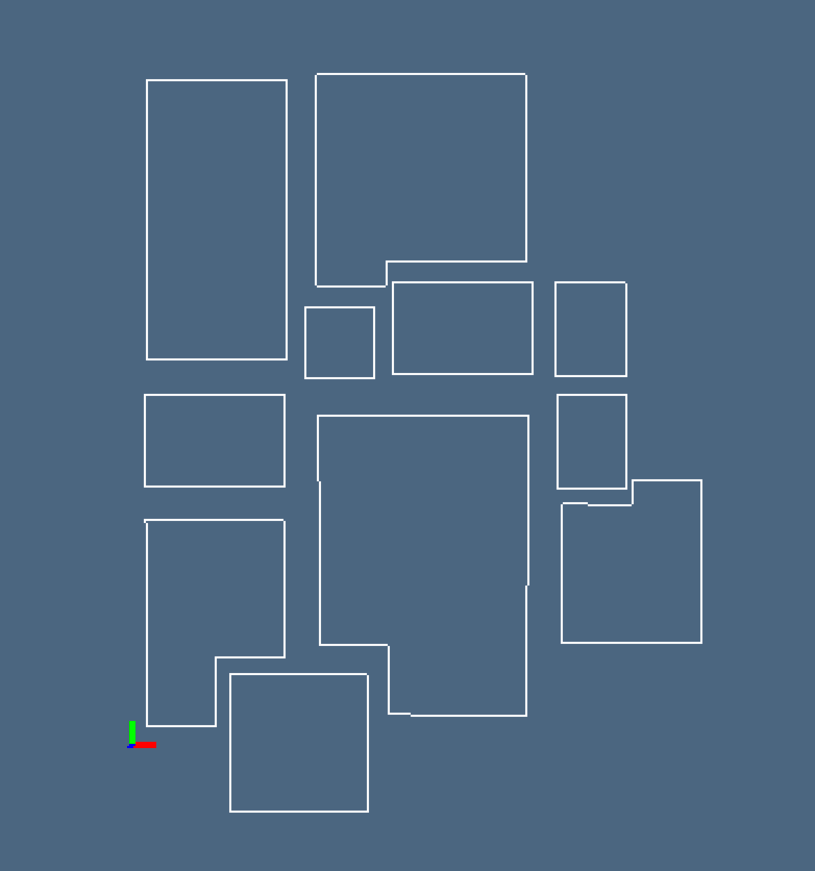
\includegraphics[height=0.243\linewidth,width=0.243\linewidth]{images/plan1} 
   
\includegraphics[height=0.243\linewidth,width=0.243\linewidth]{images/plan2} 
   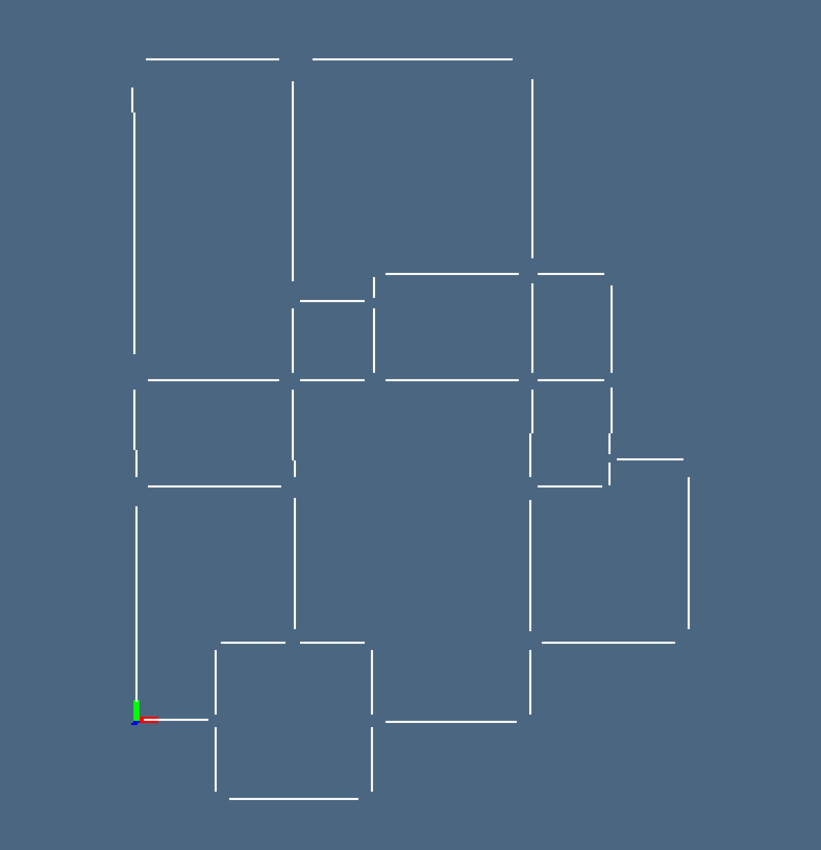
\includegraphics[height=0.243\linewidth,width=0.243\linewidth]{images/plan3} 
   \caption{(a) LAR drawing as close polylines: (b) exploded polylines: (c) exploded 2-cells: (d) exploded 1-cells.}
   \label{fig:plan2D}
\end{figure}

\paragraph{Subdivide the 1-cells of the concept plan}
The input to \texttt{bUnit\_to\_eEiP}, to compute the 1D external envelope and interior partitions starting from 2D from building units, is given below.

%-------------------------------------------------------------------------------
@D Subdivide the 1-cells
@{def bUnit_to_eEiP(FV,EV):
	""" Subdivide the 1-cells. 
	Return external envelope and interior partitions """
	eE = lar2boundaryEdges(FV,EV)
	iP = lar2InteriorEdges(FV,EV)
	return eE,iP
@}
%-------------------------------------------------------------------------------

\paragraph{Boundary cells ($2D\to 1D$) computation}
The computations of boundary cells is executed by calling the \texttt{boundaryCells} from the \texttt{larcc} module.

%-------------------------------------------------------------------------------
@D Boundary cells ($2D\to 1D$) computation
@{def lar2boundaryEdges(FV,EV):
	""" Boundary cells computation """
	return boundaryCells(FV,EV)
@}
%-------------------------------------------------------------------------------

\paragraph{Interior partitions ($2D\to 1D$) computation}
The indices of the boundary 1-cells are returned in \texttt{boundarychain1}, and subtracted from the set $\{0,1,\ldots,|E|-1\}$ in order to return the indices of the \texttt{interiorCells}.
%-------------------------------------------------------------------------------
@D Interior partitions ($2D\to 1D$) computation
@{def lar2InteriorEdges(FV,EV):
	""" Boundary cells computation """
	boundarychain1 = boundaryCells(FV,EV)
	totalChain1 = range(len(EV))
	interiorCells = set(totalChain1).difference(boundarychain1)
	return interiorCells
@}
%-------------------------------------------------------------------------------


\begin{figure}[htbp] %  figure placement: here, top, bottom, or page
   \centering
   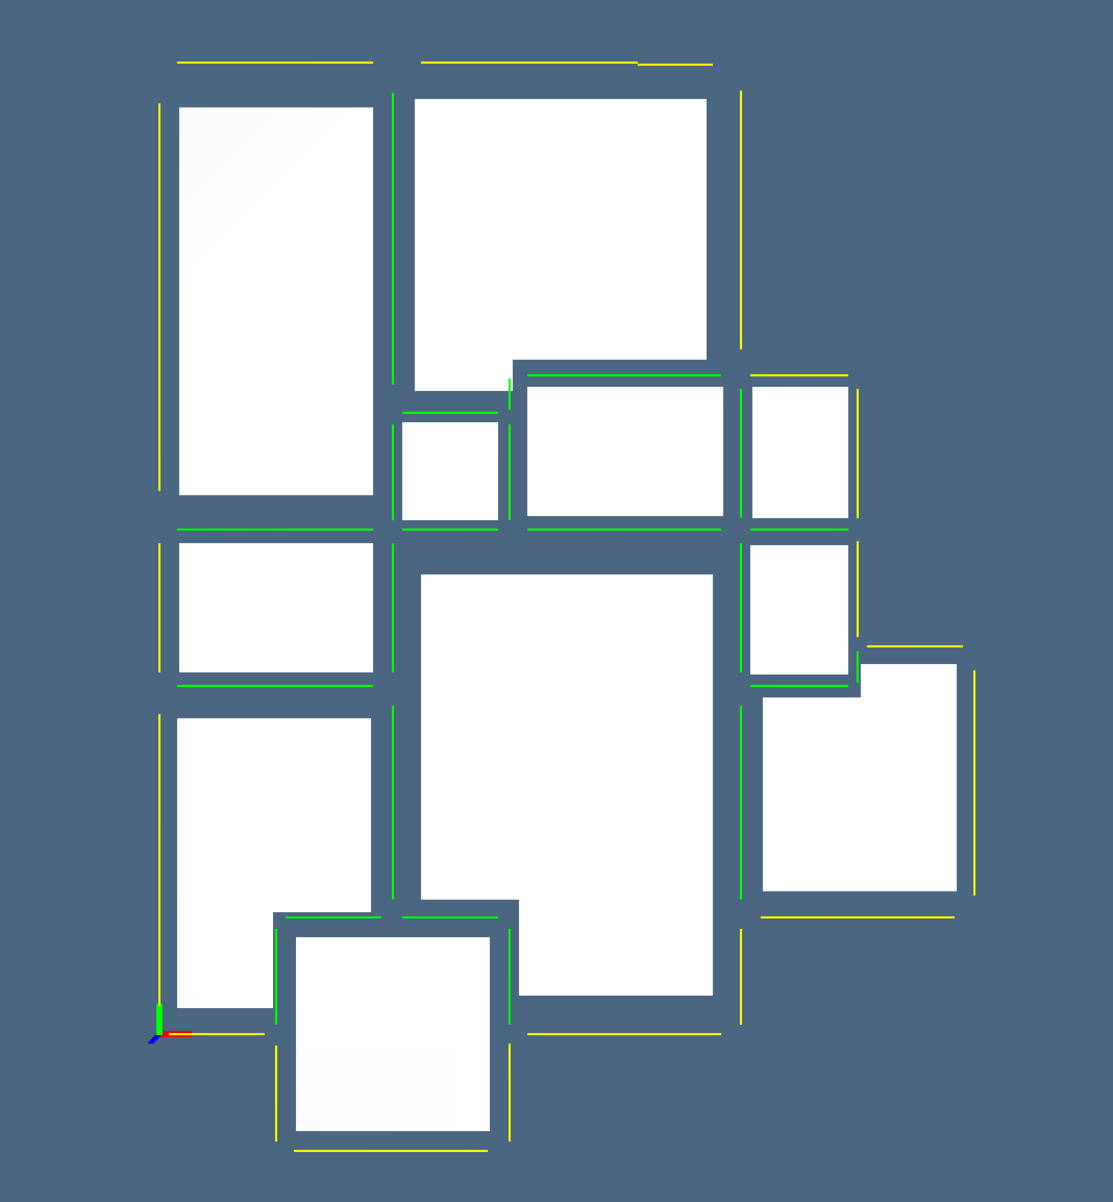
\includegraphics[height=0.325\linewidth,width=0.325\linewidth]{images/plan4} 
   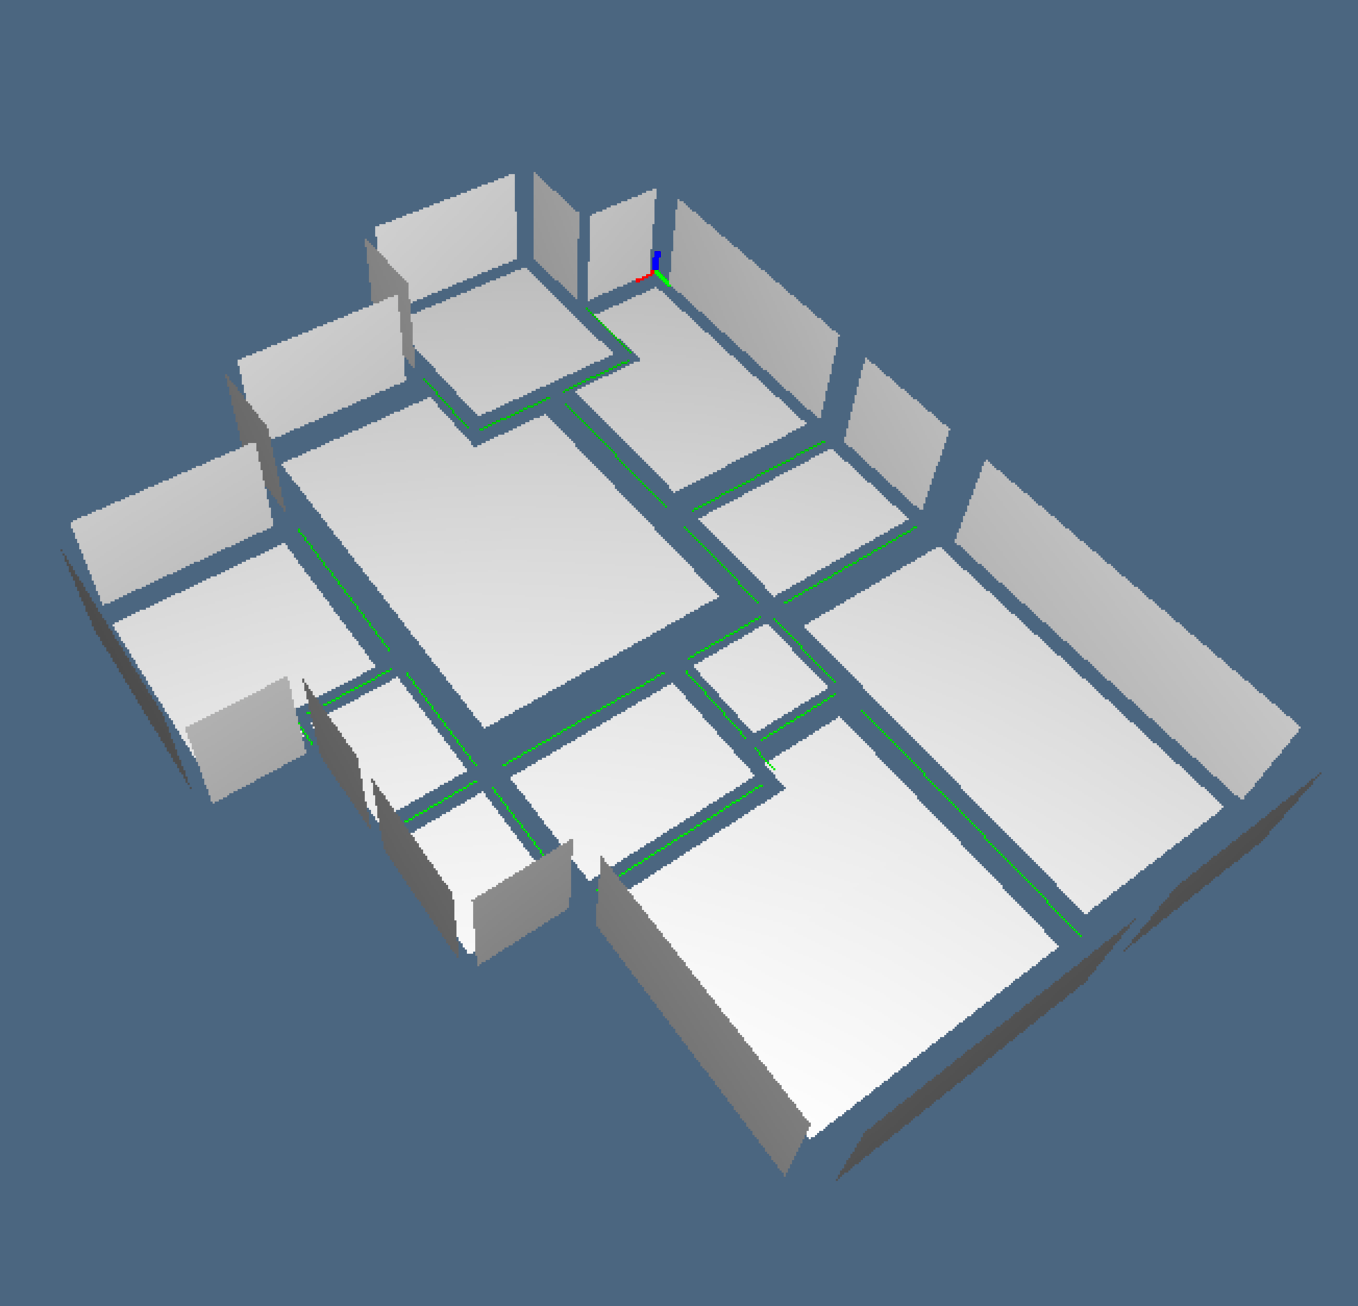
\includegraphics[height=0.325\linewidth,width=0.325\linewidth]{images/plan5} 
   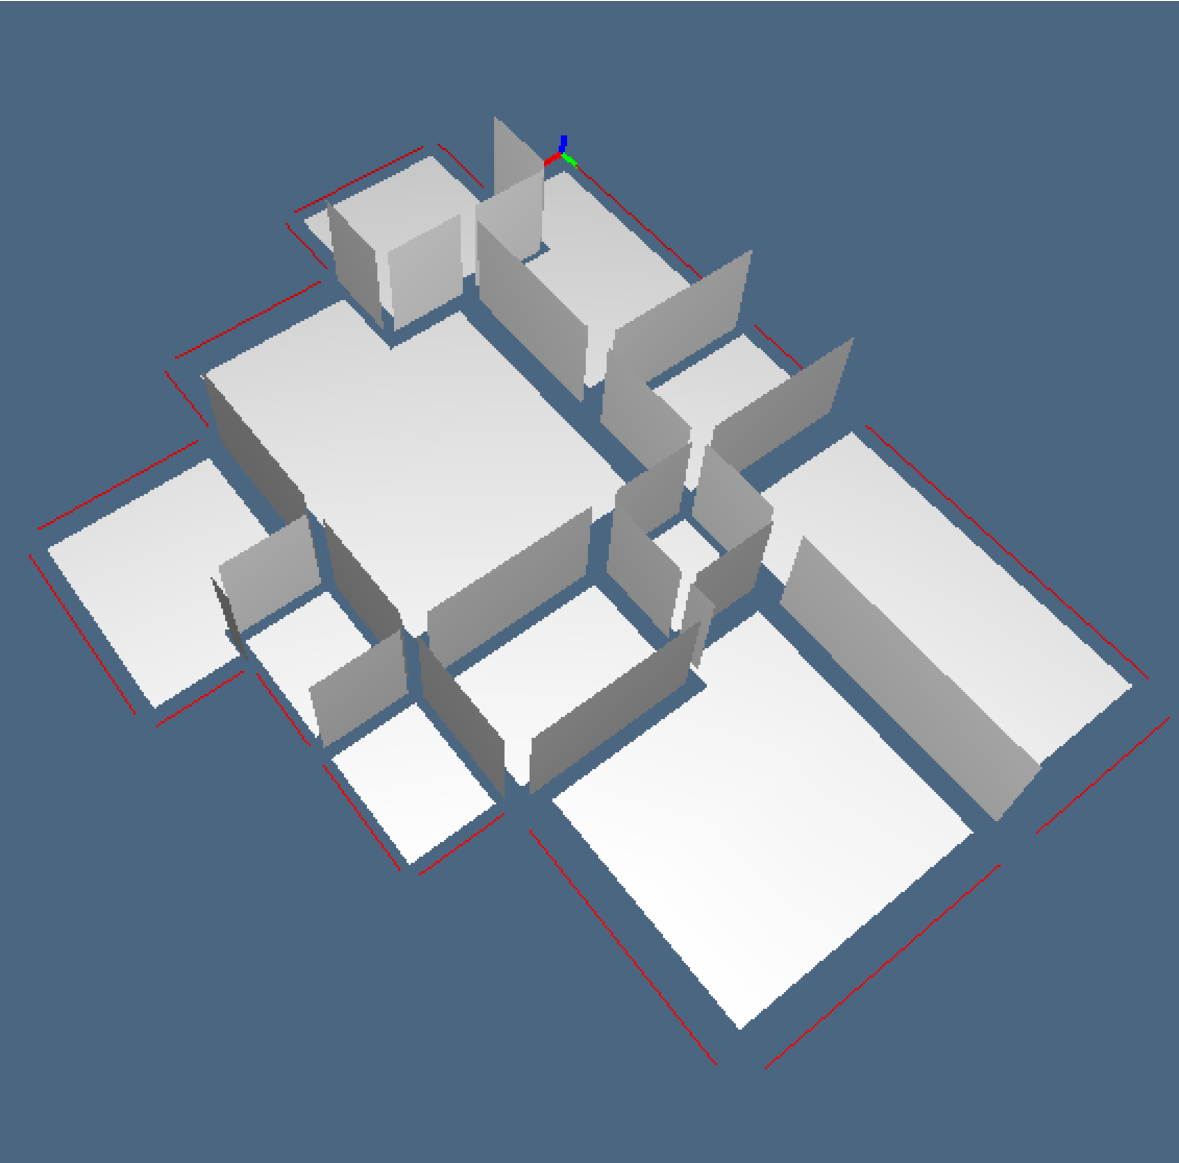
\includegraphics[height=0.325\linewidth,width=0.325\linewidth]{images/plan6} 
   \caption{(a) 2-cells, interior 1-chain (green), boundary 1-chain (red): (b) boundary 2-chain: (c) interior 2-chain.}
   \label{fig:plan2.5D}
\end{figure}


\subsubsection{Geometric aggregation of building units}

Several methods can be used to to aggregate the LAR models \texttt{[V,CV]} and  \texttt{[W,CW]} of two building units into one single structure. The method provided by the \texttt{movePoint2point(twoModels)} function aggregates the vertices of two models after having applied a translation \texttt{t()} to the second set of vertices (\texttt{W}). The translation vector is computed as vector difference of \texttt{pointQ}
and \texttt{pointP}.

\paragraph{Move : $Model \times Model \to Model$ operator}
%-------------------------------------------------------------------------------
@D Move ($P\to Q$) operator
@{def movePoint2point(twoModels):
	""" Move (P -> Q) operator """
	def movePoint2point0(pointP):
		def movePoint2point1(pointQ):
			[V,CV], [W,CW] = twoModels
			mat = t( *DIFF([pointP,pointQ]) )
			[W,CW] = larApply(mat)([W,CW])
			print "\n W =",W
			print "\n CW =",CW
			n = len(V)
			return [ V+W, CV+[[w+n for w in REVERSE(cell)] for cell in CW] ] 
		return movePoint2point1	
	return movePoint2point0
@}
%-------------------------------------------------------------------------------

\begin{figure}[htbp] %  figure placement: here, top, bottom, or page
   \centering
   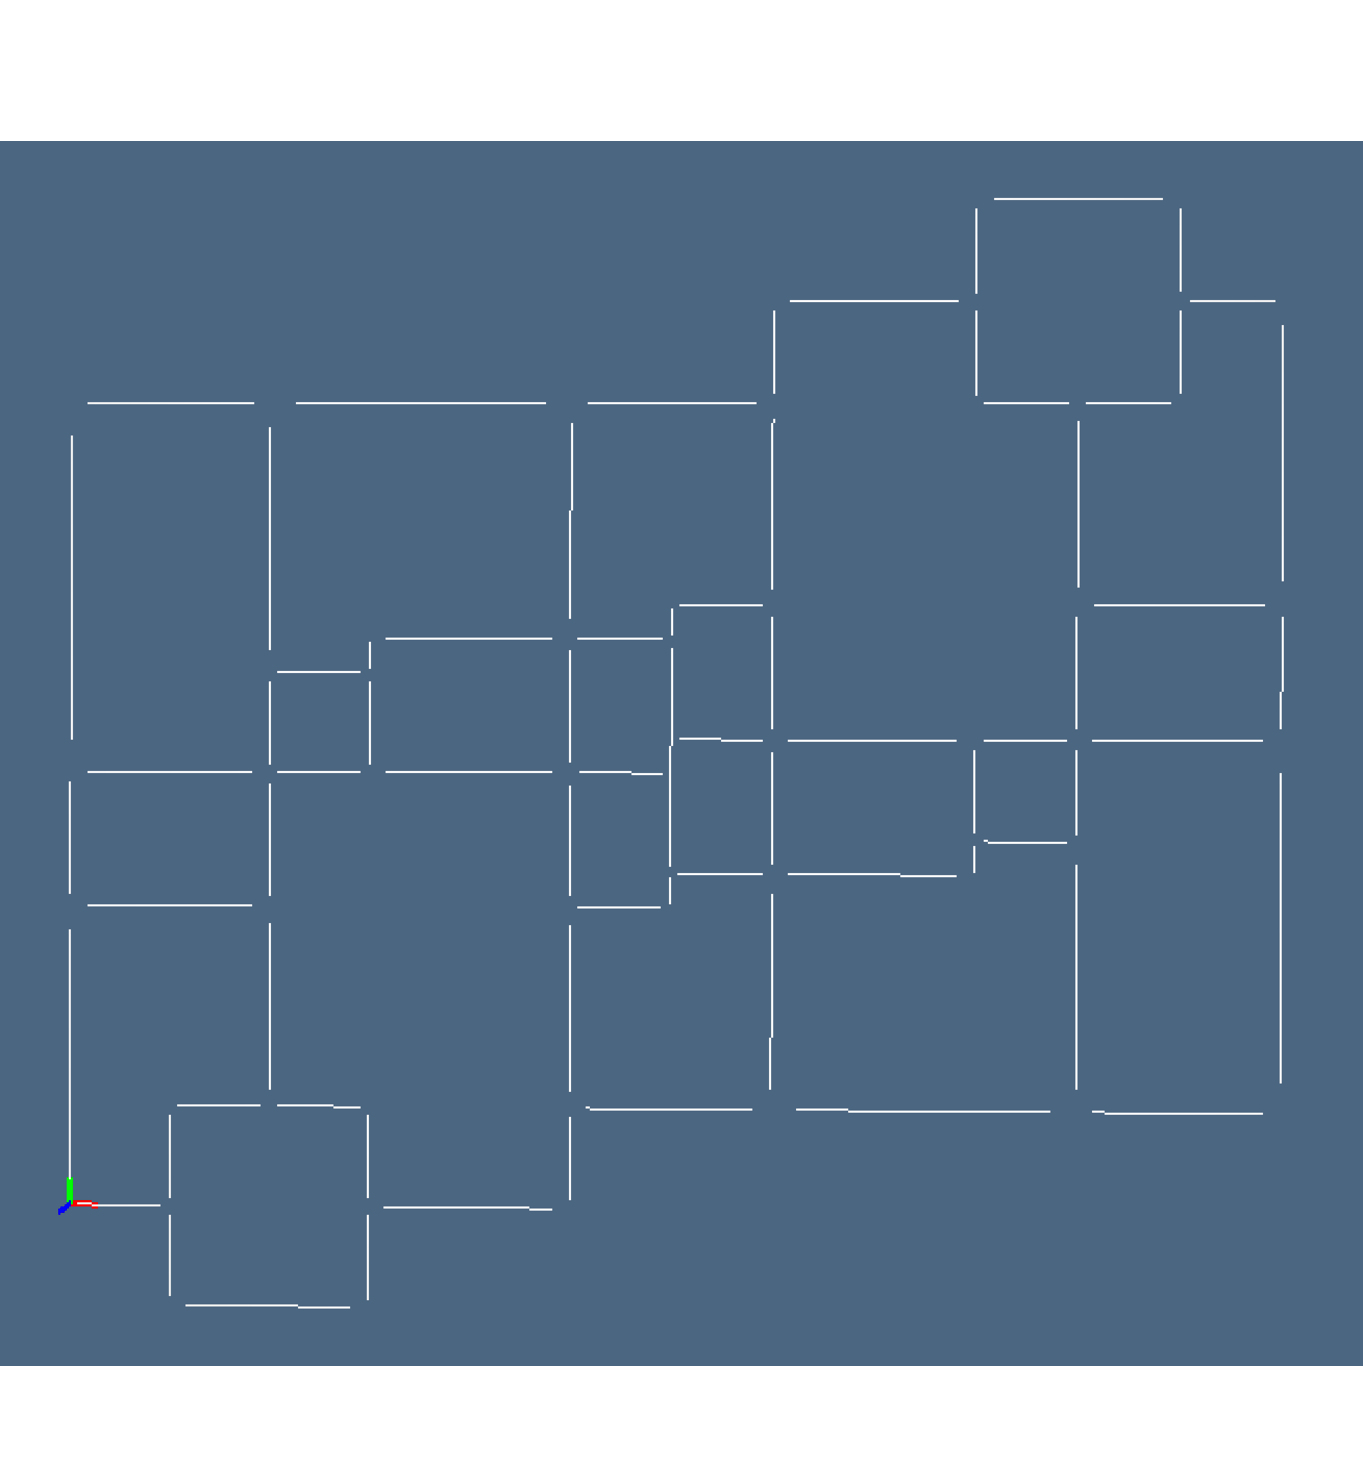
\includegraphics[width=0.33\linewidth]{images/planpair} 
   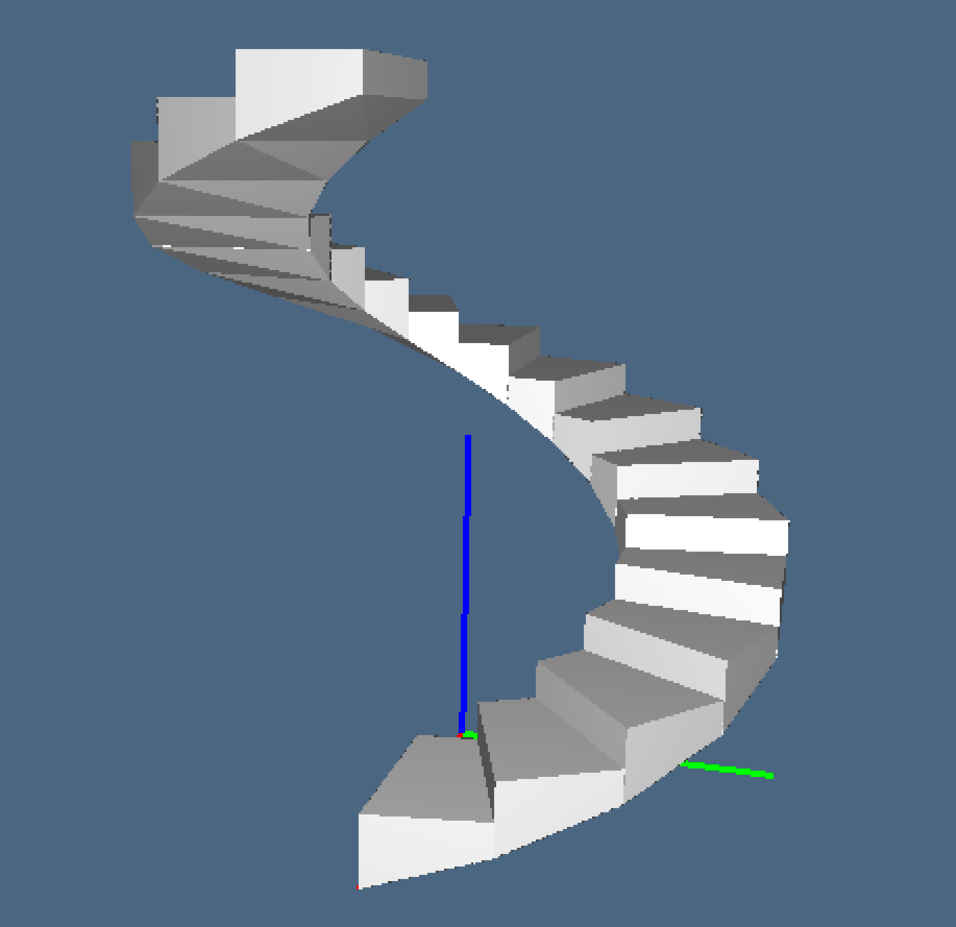
\includegraphics[width=0.3\linewidth]{images/spiralstair} 
   \caption{Concept design: (a) aggregation of two building units; (b) fully parametric spiral stair.}
   \label{fig:concept1}
\end{figure}

\paragraph{Parametric spiral stair}

A fully parametric \texttt{spiralStair} functions is given below, where the major and minor radiuses \texttt{R} and \texttt{r}, the step \texttt{riser}, the spiral \texttt{pitch}, i.e.~the distance between two turns, the real number of turns \texttt{nturns} and the number of \texttt{steps} for every $2\pi$ angle can be user-specified.

%-------------------------------------------------------------------------------
@D Trasform a solid helicoid into a spiral stair
@{def spiralStair(width=0.2,R=1.,r=0.5,riser=0.1,pitch=2.,nturns=2.,steps=18):
	V,CV = larSolidHelicoid(width,R,r,pitch,nturns,steps)()
	W = CAT([[V[k],V[k+1],V[k+2],V[k+3]]+
		[SUM([V[k+1],[0,0,-riser]]),SUM([V[k+3],[0,0,-riser]])]
		for k,v in enumerate(V[:-4]) if k%4==0])
	for k,w in enumerate(W[:-12]):
		if k%6==0: W[k+1][2] = W[k+10][2]; W[k+3][2] = W[k+11][2]
	nsteps = len(W)/12
	CW =[SUM([[0,1,2,3,6,8,10,11],[6*k]*8]) for k in range(nsteps)]
	return W,CW
	
VIEW(STRUCT(MKPOLS(spiralStair())))
VIEW(STRUCT(MKPOLS(spiralStair(0.1))))
@}
%-------------------------------------------------------------------------------


\subsubsection{Floor assembly of apartment building}

\begin{figure}[htbp] %  figure placement: here, top, bottom, or page
   \centering
   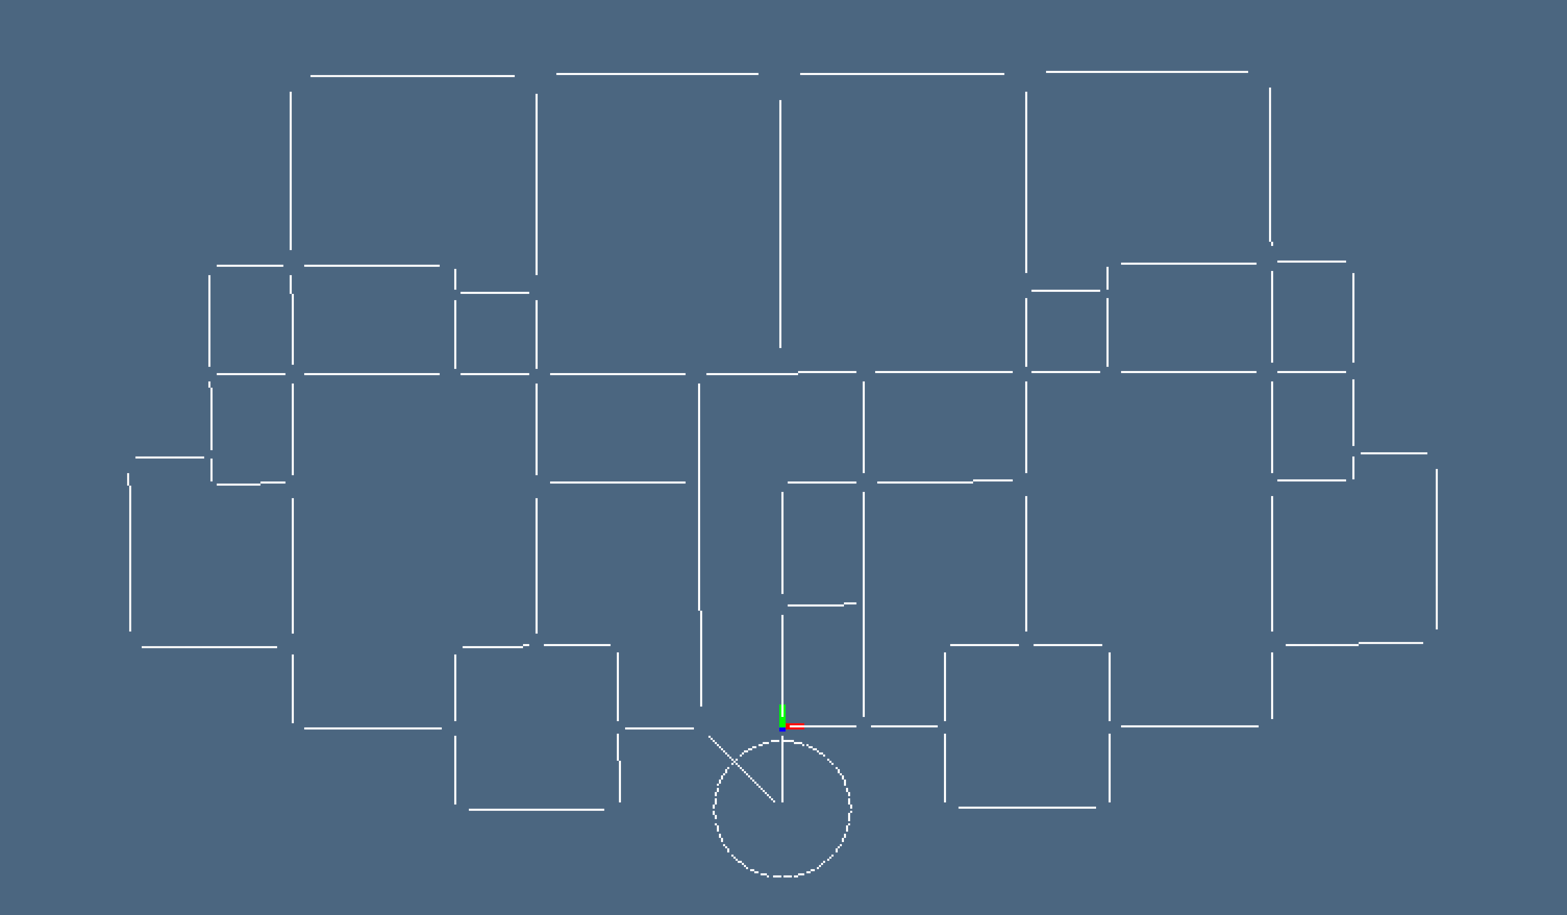
\includegraphics[width=0.6\linewidth]{images/plan2d} 
   \caption{Concept design: (a) aggregation of two building units; (b) fully parametric spiral stair.}
   \label{fig:concept1}
\end{figure}

\paragraph{Typical floor assembly of apartment block}

%-------------------------------------------------------------------------------
@O test/py/architectural/test04.py
@{""" D LAR model input and handling """
@< Initial import of modules @>
from architectural import *
from boolean import *
@< Input of LAR architectural plan @>
V,FV = larApply(t(3,0))(dwelling)
print "\n V,FV =",V,FV
VIEW(EXPLODE(1.2,1.2,1)(MKPOLS(dwelling)))
dwelling = Struct([ t(3,0), dwelling ])
V1 = [[0,0],[3,0],[3,4.5],[0,4.5],[3,9],[0,9],[3,13],[-3,13],[-3,0],[0,-3]]
FV1 = [[0,1,2,3],[3,2,4,5],[0,3,5,4,6,7,8,9]]
landing = V1,FV1
stair = spiralStair(width=0.2,R=1.5,r=0.25,riser=0.1,pitch=4.,nturns=1.75,steps=36)
stair = larApply(r(0,0,PI/4))(stair)
# stair = larDisk([1.5,1.75*PI])()
# stair = larApply(r(PI/4))(stair)
stair = larApply(t(0,-3))(larCircle(2.5)())
plan = Struct([stair,landing,dwelling,s(-1,1),dwelling])
assembly2D = evalStruct(plan)
VIEW(EXPLODE(1.2,1.2,1)(CAT(AA(MKPOLS)(assembly2D))))
assembly1D = TRANS(CONS([S1,COMP([AA(face2edge),S2])])(TRANS(assembly2D)))
VIEW(EXPLODE(1.2,1.2,1)(CAT(AA(MKPOLS)(assembly1D))))
@}
%-------------------------------------------------------------------------------


\paragraph{Spatial beams and frames}
%-------------------------------------------------------------------------------
@D Spatial beams and frames
@{

@}
%-------------------------------------------------------------------------------
\subsection{Quick BIM}
%-------------------------------------------------------------------------------
1 column
%-------------------------------------------------------------------------------
\subsection{Introducing time}
%-------------------------------------------------------------------------------
1.5 column
%-------------------------------------------------------------------------------
%===============================================================================
\section{The computational framework}\label{sec:library}
%===============================================================================
%-------------------------------------------------------------------------------
\subsection{ABC: a set of classes}
%-------------------------------------------------------------------------------
1 column
%-------------------------------------------------------------------------------
\subsection{Some specialised methods}
%-------------------------------------------------------------------------------
2 column
%-------------------------------------------------------------------------------
\subsection{Zero install: working in the browser}
%-------------------------------------------------------------------------------
0.5 column
%-------------------------------------------------------------------------------
%-------------------------------------------------------------------------------
\subsection{Exporting the library}
%-------------------------------------------------------------------------------

@O lib/py/architectural.py
@{@< Initial import of modules @>
@< From faces FV to list of edges EV @>
@< Subdivide the 1-cells @>
@< Boundary cells ($2D\to 1D$) computation @>
@< Interior partitions ($2D\to 1D$) computation @>
@< Move ($P\to Q$) operator @>
@< Subdivide the 1-cells of the concept plan @>
@< Trasform a solid helicoid into a spiral stair @>
@}
%===============================================================================
\section{Conclusion}\label{sec:conclusion}
%===============================================================================
%-------------------------------------------------------------------------------
\subsection{The state of the art}
%-------------------------------------------------------------------------------
0.5 column
%-------------------------------------------------------------------------------
\subsection{What next}
%-------------------------------------------------------------------------------
0.5 column

\bibliographystyle{amsalpha}
\bibliography{architectural}
1.5 column
= 10 pages

%-------------------------------------------------------------------------------
%===============================================================================
\appendix
\section{Appendix}
\section{Utility functions}
%===============================================================================

\paragraph{Initial import of modules}

%-------------------------------------------------------------------------------
@D Initial import of modules
@{from pyplasm import *
from scipy import *
import os,sys
""" import modules from larcc/lib """
sys.path.insert(0, 'lib/py/')
from lar2psm import *
from simplexn import *
from larcc import *
from largrid import *
from mapper import *
from boolean import vertexSieve
@}
%-------------------------------------------------------------------------------

\section{Tests}


\paragraph{Concept design}

%-------------------------------------------------------------------------------
@O test/py/architectural/test01.py
@{@< Initial import of modules @>
from architectural import *
@< Input of LAR architectural plan @>
# VIEW(STRUCT(AA(POLYLINE)(lar2polylines (model))))
# VIEW(EXPLODE(1.2,1.2,1)(AA(POLYLINE)(lar2polylines (model))))
bU = AA(SOLIDIFY)(AA(POLYLINE)(lar2polylines (dwelling)))
# VIEW(EXPLODE(1.2,1.2,1)(bU))
EV = face2edge(FV)
VIEW(EXPLODE(1.2,1.2,1)(MKPOLS((V,EV))))

eE,iP = bUnit_to_eEiP(FV,EV)
modEe1D = V, [EV[e] for e in eE]
modIp1D = V, [EV[e] for e in iP]
eE1D = AA(COLOR(RED))(MKPOLS(modEe1D))
iP1D = AA(COLOR(GREEN))(MKPOLS(modIp1D))

VIEW(EXPLODE(1.2,1.2,1)(eE1D))
VIEW(EXPLODE(1.2,1.2,1)(iP1D))
VIEW(STRUCT(bU + iP1D + eE1D))
VIEW(EXPLODE(1.2,1.2,1)(bU + iP1D + eE1D))

floorHeight = larIntervals([1])([4])
modIp2D = larModelProduct([ modIp1D, floorHeight ])
modEe2D = larModelProduct([ modEe1D, floorHeight ])

VIEW(EXPLODE(1.2,1.2,1)(bU + MKPOLS(modIp2D) + eE1D))
VIEW(EXPLODE(1.2,1.2,1)(bU + iP1D + MKPOLS(modEe2D)))
VIEW(EXPLODE(1.2,1.2,1)(bU + MKPOLS(modIp2D) + MKPOLS(modEe2D)))
@}
%-------------------------------------------------------------------------------



%-------------------------------------------------------------------------------
@O test/py/architectural/test02.py
@{@< Initial import of modules @>
from architectural import *
@< Input of LAR architectural plan @>
(W,FW) = larApply(s(-1,-1))(dwelling)
(V,FV) = dwelling
(V,FV) = movePoint2point([ (V,FV),(W,FW) ])(V[20])(W[25])
EV = face2edge(FV)
VIEW(EXPLODE(1.2,1.2,1)(MKPOLS((V,EV))))
@}
%-------------------------------------------------------------------------------

%# PROD([[h]*(n+1),range(n+1)])
%# extrude
%# def larQuote(measures)


%-------------------------------------------------------------------------------
@O test/py/architectural/test03.py
@{def plan2mockup(model,h,n):
	V,FV = model
	EV = face2edge(FV)
	eE,iP = bUnit_to_eEiP(FV,EV)
	modEe1D = V, [EV[e] for e in eE]
	modIp1D = V, [EV[e] for e in iP]
	modVert0D = larExtrude1( VOID, 6*[1] )
	modVert1D = larExtrude1( VOID, 6*[1] )
	horParts = larModelProduct([ model, modVert0D ])
	
VIEW(EXPLODE(1.2,1.2,1)(MKPOLS((X,FX))))
@}
%-------------------------------------------------------------------------------




\end{document}
